% !TEX root = ./thesis.tex

\chapter{Evaluation}
\label{ch:eval}

Finding a definite good evaluation method for unsupervised models is a long-standing and inherent problem.


\section{Evaluation dataset}
\subsection{Data collection}

Access to large amount of training data is crucial for applying deep learning models.
Successes of deep learning on image recognition and segmentation tasks can be attributed to existence of large research datasets as ILSVRC and Places365 \cite{ILSVRC15, Zhou2016} containing millions of labeled images.
Machine translation, NLP tasks \cite{Karpathy2014, Kim2014} often rely on low-dimensional word embedding models.
Such models, as for example as word2vec or Glove \cite{Mikolov2013, pennington2014glove}, are trained on terabytes of textual data.
Deep reinforcement models might use existing gaming engines to generate required training data "on the go".
As, for example Google DeepMind team uses Atari 2D games to generate data for Q-learning \cite{Mnih2013}.

For the purpose of this research we collect visual data using the ViZDoom AI research platform \cite{Kempka2016}.
ViZDoom is a Doom-based platform for reinforcement learning.
It provides access to raw visual data from the Doom gaming engine.
Doom is a first-person shooter (FPS) computer game utilizing 3D graphics.
In context of our research the ViZDoom platform allows automatic visual data generation and collection.
Example of the output image is shown on figure \ref{fig:doom}.

We created multiple Doom maps specifically for our task using the Slade \cite{Slade3} software.
Created maps provide high diversity of textures for better discrimination between images, captured from different positions on the map.
Other reason for diverse structures on the map is to explicitly brake symmetry of the map.
Symmetric maps look alike from different player positions which leads to entangled manifolds in feature space.
Such position tend to be encoded with the same values of sparse features.
This represents a difficulty for evaluation and comparison of quality of sparse features.

We record multiple movement trajectories on each map.
More specifically, we record 10000-300000 consecutive images of unstructured movement of the player on the map for training purposes.
In addition to that, we record movement along well defined structured trajectories as a "circle" or an "eight" for model evaluation and comparison of quality of extracted features.


\begin{figure}
\centering
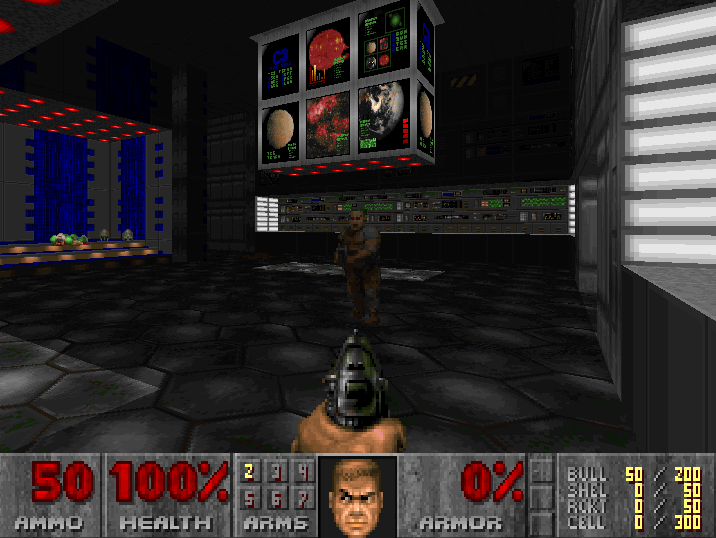
\includegraphics[width=.80\textwidth]{doom.png} %{CS0031}
\caption{Example of DoomII image collected with ViZDoom \cite{Kempka2016}.}
\label{fig:doom}
\end{figure}

\subsection{Dataset description}

We collect multiple sets of visual data with varying complexity of players movement.
We can specify next 3 classes of trajectories used either for training or evaluation:
\begin{itemize}
  \item Continuous closed trajectory without intersection. A circular movement is one example of such trajectory.
  \item Continuous closed trajectory with intersection. An \text{eight} is an example of such trajectory.
  \item Continuous random movement across the environment (map).
\end{itemize}

Furthermore, we introduce multiple complexity levels of movement across trajectories by reducing degrees of freedom of such movements:
\begin{itemize}
  \item Most restricted. Only movement along a single axis at a time is possible. This category includes movements across rectangular trajectories while maintaining fixed direction of the view or changing the direction of the view while standing still. This category provides includes trajectories of the lowest complexity.
  \item Less restricted. Multiple degrees of freedom at a time allowed. For example, movement along multiple axis facing one direction or forward movement while changing the direction of the view.
  \item Free movement across the map with no restrictions.
\end{itemize}


\subsection{Data format}

We collect RGBD images from the 3D engine. Each image has resolution of 160 by 120 pixels. Each pixel is describe by 3 color channels and a single distance channel. Each channel can take a discrete value between 0 and 255 including. This format results in 76800 dimensional inputs.

\section{Model comparison}



\section{Predictive evaluation}

Evaluation of the performance of unsupervised models is inherently difficult.
Discriminative models typically use well-defined metrics with clear quantifiable outputs, as classification accuracy, F-measure etc. Unsupervised models generally have no access to such metrics.
Solutions for some under-defined objectives, as finding image super-resolution or generating new data samples, can be evaluated by involving manual human grading, which is costly and time-consuming \cite{Dahl2017, Goodfellow2014}.
Other models rely on the primary learning objective, which is not necessarily representative of the actual model performance. As, for example, minimizing MSE for image comparison can result in low-quality blurry results, or matching certain characteristics of natural probability distribution in a generative process does not guarantee realistically looking generated data \cite{Li2015, Mathieu2015}. At last, some unsupervised learning techniques can be evaluated through performance on real world tasks by showing, that results of unsupervised learning can improve performance of discriminative models. For example, reusing network weights of denoising and contractive autoencoders led to improved classification results \cite{Rifai2011, Vincent2010}, as well reusing weights of word embeddings \cite{NIPS2013_5021} led to increased performance on a number of natural language processing tasks.

In context of this work we would like to have access to a concise measure for comparison of model designs.
Primary objective of an autoencoder -- good reconstruction of the input image -- is not very descriptive, since it makes no assumption about the spatial characteristics of the extracted features. Nevertheless, we provide our reconstruction loss values with the experiments.

We are going to use \textit{predictive evaluation} as a main mean of model comparison from perspective of spatial feature extraction. With the predictive objective we would like to evaluate the quality of extracted spatial features. We do that by considering local resemblance of the manifold to an euclidean space. But, since we are working with unlabeled data another assumption is required. Namely, for any trajectory of actors movement we expect, that the best approximation of the transition between current and next step to be equivalent to the transition between previous and current step (when only last two frames are available for performing the prediction). We, therefore try to predict spatial position of the player on the next step on the manifold calculating it as $\hat{x}_{t+1} = x_t + (x_t- x_{t-1})$. Figure \ref{fig:m_pred} illustrates the process. Since different models have different deformations of manifold space and, therefore, might differ in terms of absolute values of the $L_2$ loss between predicted and actual location $L_2(\hat{x}_{t+1}, x_{t+1})$, we use relative improvement as a reference. We compare the improvement of prediction over a naive prediction $\tilde{x}_{t+1} = x_t$.

Note, that similar technique is used as a model regularization. Yet, predictive regularization is applied as a reconstruction error and does not have direct effect on the predictive metric. For example, an decoder of large enough capacity can have very low reconstruction error of both actual encoding $x_{t+1}$ and predictive encoding $\hat{x}_{t+1}$, but low score of predictive evaluation. This can happen when two prototypes in the embedding space $x_{t+1}$ and $\hat{x}_{t+1}$ have distinct difference, but are still reconstructed as alike images due to overfitting appearing in the decoder network.

% TODO: finish it: analyze the overfitting in the decoder network in relation to predictive evaluation

\subsection{Backbone model comparison}


\subsection{Regularization}


\subsection{Dataset complexity}


\subsection{Relevance of depth information}




\section{Loop closure detection}

Compare to \cite{Xia2016} on Freiburg2 dataset for loop closure detection.

\section{Manifold construction}

Compare to \cite{Jaderberg2015} in terms of how valuable the representation comparing to their results.

\section{Topology reconstruction}

Shall be removed(
